\documentclass[UTF8]{ctexart}
\usepackage[table]{xcolor}
\usepackage{bm}
\usepackage{amssymb}
\usepackage{mathtools}
\usepackage{amsmath}
\usepackage{float}
\usepackage{rotating}
\usepackage{booktabs}
\usepackage{pdfpages}
\usepackage{subfigure}
\usepackage{mathtools}
\usepackage{amsmath}
\usepackage{listings}
\usepackage{fancybox}
%\usepackage{xcolor}
%\usepackage{colortbl}
\usepackage{diagbox}
\usepackage{amssymb}
\usepackage{warpcol}
\usepackage{lscape}
\usepackage[framemethod=tikz]{mdframed}
\usepackage{longtable,booktabs}
\definecolor{ocre}{RGB}{243,102,25}
\definecolor{mygray}{RGB}{243,243,244}

\title{\heiti 最优化第十七次作业}
\author{\kaishu 张晋15091060}
\begin{document}
\maketitle

\begin{enumerate}
\item[7.9]
函数图像如下:
\begin{figure}[H]
\centering
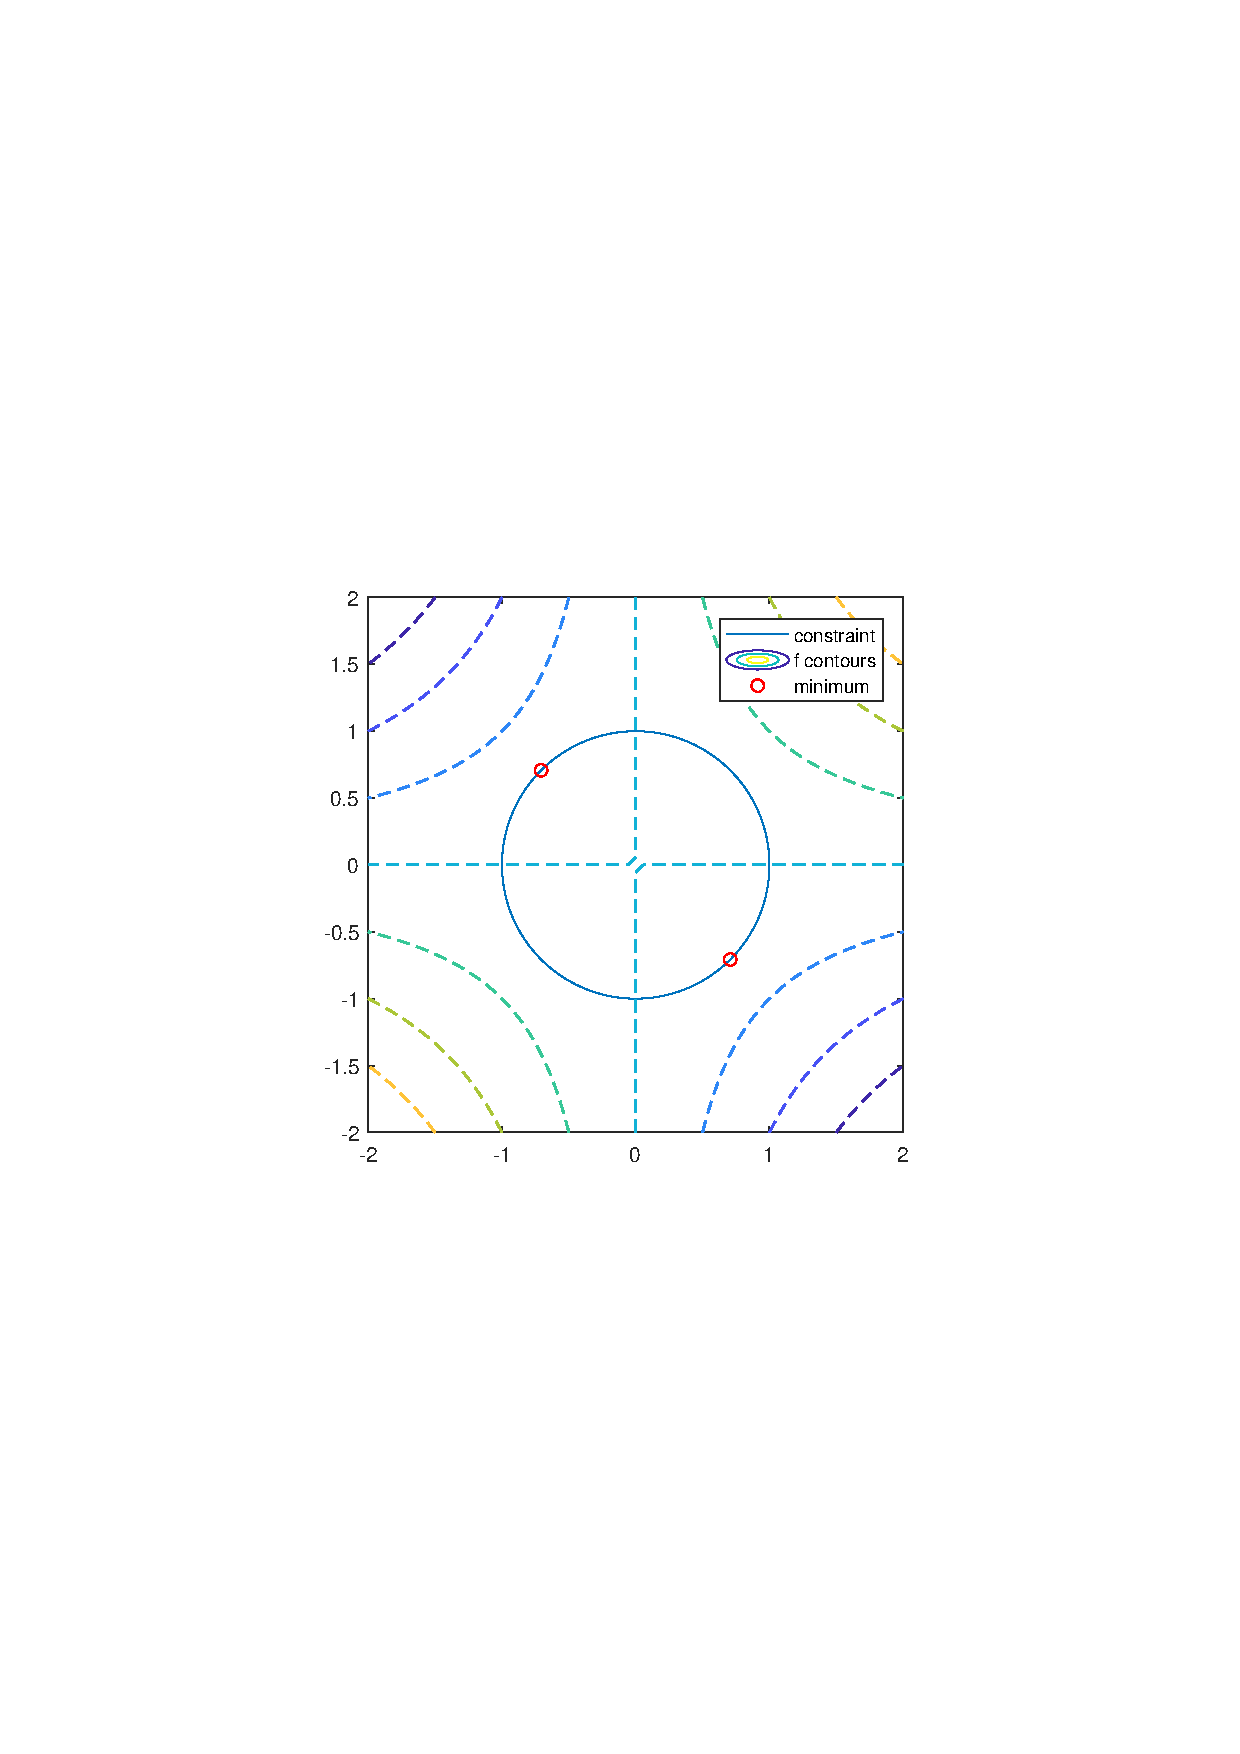
\includegraphics[width=8cm]{1.pdf}
\end{figure}

\[\mathcal{L}(\bm{x},\lambda)=x_1x_2+\lambda(x_1^2+x_2^2-1)\]

\[\nabla_{\bm{x}}\mathcal{L}(\bm{x},\lambda)=\begin{bmatrix}
2\lambda x_1+x_2\\
x_1+2\lambda x_2\\
\end{bmatrix}\]

\[\nabla_{\bm{x}}^2\mathcal{L}(\bm{x},\lambda)=\begin{bmatrix}
2\lambda &1\\
1&2\lambda
\end{bmatrix}\]

\subsection*{KKT条件:}
\begin{align}
2\lambda x_1+x_2&=0\\
x_1+2\lambda x_2&=0\\
x_1^2+x_2^2-1&=0
\end{align}

解以上方程得:
\[\bm{x}^{(1)}=(\dfrac{\sqrt{2}}{2},\dfrac{\sqrt{2}}{2})^T,\qquad \lambda^{(1)}=-\dfrac{1}{2}\]
\[\bm{x}^{(2)}=(-\dfrac{\sqrt{2}}{2},\dfrac{\sqrt{2}}{2})^T,\qquad \lambda^{(2)}=\dfrac{1}{2}\]
\[\bm{x}^{(3)}=(\dfrac{\sqrt{2}}{2},-\dfrac{\sqrt{2}}{2})^T,\qquad \lambda^{(3)}=\dfrac{1}{2}\]
\[\bm{x}^{(4)}=(-\dfrac{\sqrt{2}}{2},-\dfrac{\sqrt{2}}{2})^T,\qquad \lambda^{(4)}=-\dfrac{1}{2}\]

\subsection*{对$\bm{x}^{(1)}:$}
\[\nabla_{\bm{x}}^2\mathcal{L}(\bm{x}^{(1)},\lambda)=\begin{bmatrix}
-1 &1\\
1&-1
\end{bmatrix}=\bm{W}_1\]
\[G(\bm{x}^{(1)},\lambda^{(1)})=k(1,-1)^T=\bm{p}_1\]
\[{\bm{p}_1}^TW\bm{p}_1=-4k^2<0\]

故$\bm{x}^{(1)}$非局部最优解。




\subsection*{对$\bm{x}^{(2)}:$}
\[\nabla_{\bm{x}}^2\mathcal{L}(\bm{x}^{(2)},\lambda)=\begin{bmatrix}
1 &1\\
1&1
\end{bmatrix}=\bm{W}_2\]
\[G(\bm{x}^{(2)},\lambda^{(2)})=k(1,1)^T=\bm{p}_2\]
\[{\bm{p}_2}^TW\bm{p}_2=4k^2>0\]

故$\bm{x}^{(2)}$是局部最优解。



\subsection*{对$\bm{x}^{(3)}:$}
\[\nabla_{\bm{x}}^2\mathcal{L}(\bm{x}^{(3)},\lambda)=\begin{bmatrix}
1 &1\\
1&1
\end{bmatrix}=\bm{W}_3\]
\[G(\bm{x}^{(3)},\lambda^{(3)})=k(1,1)^T=\bm{p}_3\]
\[{\bm{p}_3}^TW\bm{p}_3=4k^2>0\]

故$\bm{x}^{(3)}$是局部最优解。


\subsection*{对$\bm{x}^{(4)}:$}
\[\nabla_{\bm{x}}^2\mathcal{L}(\bm{x}^{(4)},\lambda)=\begin{bmatrix}
-1 &1\\
1&-1
\end{bmatrix}=\bm{W}_4\]
\[G(\bm{x}^{(4)},\lambda^{(4)})=k(1,-1)^T=\bm{p}_4\]
\[{\bm{p}_4}^TW\bm{p}_4=-4k^2<0\]

故$\bm{x}^{(4)}$非局部最优解。

\textbf{综上:}该问题极小点为$\bm{x}^{(2)},\bm{x}^{(3)}$,极小值为$-0.5$

\item[7.10]
\subsection*{必要性:若$[f,C]$是凸集}
设\[\big(\bm{x}_0,f(\bm{x}_0)\big),\big(\bm{x}_1,f(\bm{x}_1)\big)\in[f,C] \]
因为$[f,C]$是凸集,那么
\[\big(\bm{x}_\theta=(1-\theta)\bm{x}_0+\theta\bm{x}_1,(1-\theta)f(\bm{x}_0)+\theta f(\bm{x}_1)\big)\in[f,C] \]
根据$[f,C]$的定义,有:
\[f(\bm{x}_\theta)\leq (1-\theta)f(\bm{x}_0)+\theta f(\bm{x}_1)\]
故$f(\bm{x})$是凸函数.

\subsection*{充分性:若$f(\bm{x})$是凸函数}
那么对$\bm{x}_0,\bm{x}_1,\bm{x}_\theta$满足
\[\big(\bm{x}_0,f(\bm{x}_0)\big),\big(\bm{x}_1,f(\bm{x}_1)\big),\big(\bm{x}_\theta,f(\bm{x}_\theta)\big)\in[f,C] \]
对$\bm{x}_\theta=(1-\theta)\bm{x}_0+\theta\bm{x}_1$,有:
\[f(\bm{x}_\theta)\leq (1-\theta)f(\bm{x}_0)+\theta f(\bm{x}_1)\]
即:
\[\big(\bm{x}_\theta,(1-\theta)f(\bm{x}_0)+\theta f(\bm{x}_1)\big)\in[f,C] \]
故有:
\[(1-\theta)\big(\bm{x}_0,f(\bm{x}_0)\big)+\theta\big(\bm{x}_1,f(\bm{x}_1)\big)\in[f,C] \]
即$[f,C]$是凸集.

\item[7.11]
\begin{enumerate}
\item
由次梯度的定义有$f(\bm{x}+\alpha \bm{h})-f(\bm{x})\geq \alpha \bm{p}^T\bm{h}$
故有:
\[\lim _{a\rightarrow 0^{+}}\dfrac {f(\bm{x}+\alpha \bm{h})-f(\bm{x})}{\alpha}\geq \bm{p}^T\bm{h}\]
\[\lim _{a\rightarrow 0^{-}}\dfrac {f(\bm{x}+\alpha \bm{h})-f(\bm{x})}{\alpha}\leq \bm{p}^T\bm{h}\]

又$f$在$\bm{x}$可微,则有
\[\lim _{a\rightarrow 0}\dfrac {f(\bm{x}+\alpha \bm{h})-f(\bm{x})}{\alpha}=\bm{h}^T\nabla f(\bm{x})\]

且由可微性的定义:
\[\nabla f(\bm{x})=\bm{p}^T\bm{h}\]
即$\bm{p}=\nabla f(\bm{x}),\quad \partial f(\bm{x})=\{\nabla f(\bm{x})\}$

\item
对于$x \in (-\infty ,0)$时,$f(x)=-x$可微,$\partial f(x)=-1$

对于$x \in (0,\infty )$时,$f(x)=x$可微,$\partial f(x)=1$

对于$x =0$时,由次梯度的定义有:$|\Delta x|\geq p \Delta x$成立,

易得$-1\leq p\leq 1$,即

\[\partial f(x) = \begin{cases}
\{-1\},& x \in (-\infty ,0)\\
\{1\},& x \in (0,\infty )\\
[-1,1],&x=0
\end{cases}\]
\end{enumerate}
\end{enumerate}
\end{document}